\newpage
\section{Aufgabe2}
\label{sec:a2}

\subsection{a)}
\label{subsec:a2a}
In der Abbildung \ref{fig:scatter} sind die beiden Populationen
$P_0$ und $P_1$ sowie die drei Projektionsgeraden:
\begin{align}
  g_1(x)=0\\
  g_2(x)=-\frac34x\\
  g_3(x)=-\frac54x
\end{align}
\begin{figure}
  \centering
  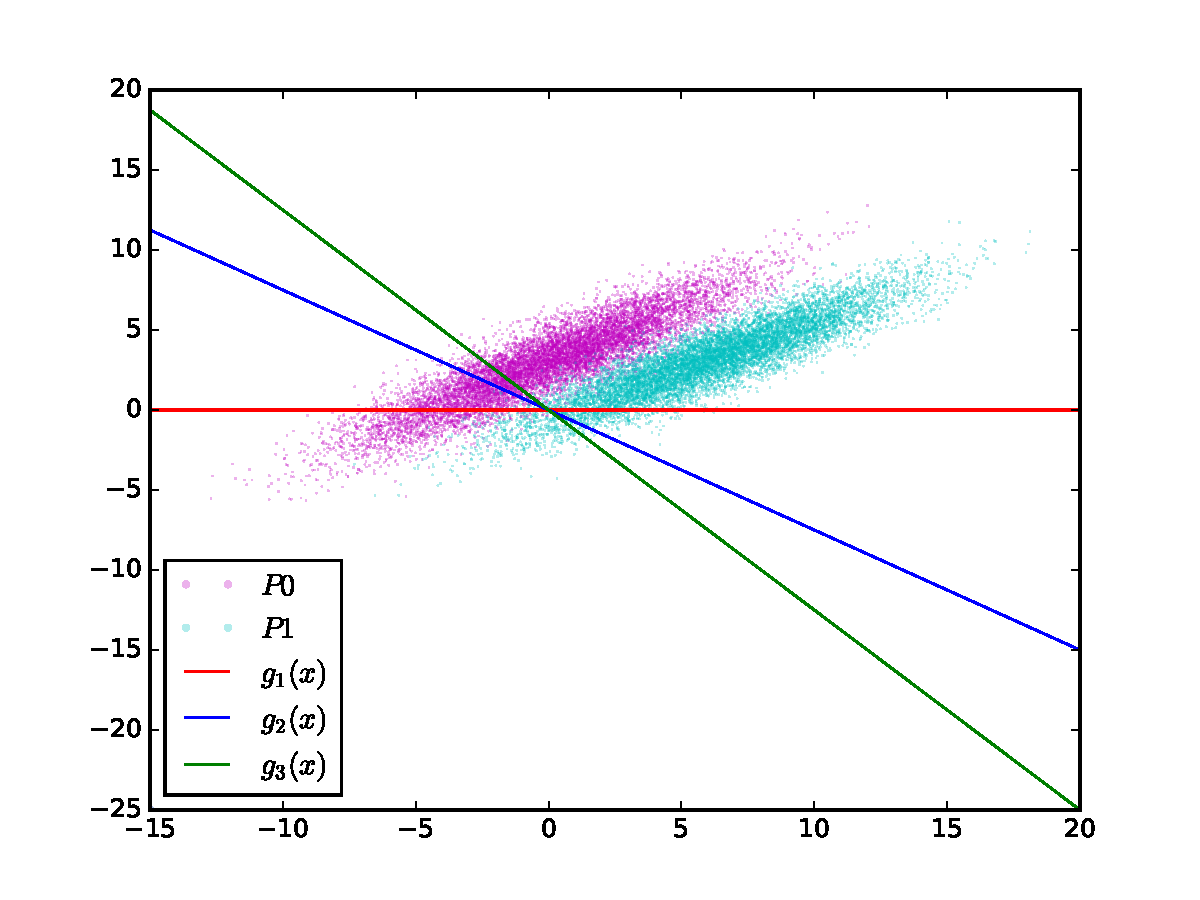
\includegraphics[width=0.7\textwidth]{scatterplot2D.pdf}
  \caption{Zweidimensionaler Scatterplot der Populationen und die
  Projektionsgeraden.}
  \label{fig:scatter}
\end{figure}
\subsection{b)}
\label{subsec:a2b}

\subsection{c)}
\label{subsec:a2c}
